%File: model.tex
%Date: Fri Jan 03 17:51:29 2014 +0800
%Author: Yuxin Wu <ppwwyyxxc@gmail.com>

\subsection{GMM}
\textbf{Gaussian Mixture Model} is commonly used in acoustic learning task such as speech/speaker recognition,
since it describes the varied distribution of all the feature vector.
GMM assumes that the probability of a feature vector $ \theta$ belonging to the model is the following:
    \[ p(\theta) = \sum_{i=1}^{K}{w_i \mathcal{N}(\mathbf{\mu}_i, \Sigma_i)}\]

  Therefore, GMM is merely a weighted combination of multivariate Gaussian distribution.
  (Actually we use diagonal covariances since the dimensions of the feature vector is independent to each other).
  GMM can describe the distribution of feature vector with several clusters, as shown in \figref{gmm-fig}
\begin{figure}[H]
  \centering
  \includegraphics[width=0.8\textwidth]{img/gmm.png}
  \caption{A Two-Dimensional GMM with Two Components\label{fig:gmm-fig}}
\end{figure}

The training of GMM is the process to find the best parameters for $ \mu_i, \Sigma_i, w_i$,
so that the model fits all the training data with maximized likelihood.
After training, the model can give the score of fitness for every input feature vector,
measuring the probability that the vector belongs to this model.

Therefore, in the task of speaker recognition, we can train a GMM for every speaker.
Then for a input signal, we extract lists of feature vectors for it, and calculate the
overall likelihood that the vectors belong to each model.
The speaker whose model fits the input best will be choosen as the answer.

Moreover, an enhancement have been done to the original GMM method.
The training of GMM first requires a random initialization of the means of
all the components. However, we can first use K-Means algorithm\cite{kmeans} to perform a clustering
to all the vectors, then use the clustered centers to initialize the training of GMM.
This enhancement can speed up the trainig, also gives a better training result.


\begin{itemize}
  \item Performance: \\
    We investigate the effect of initialization of GMM during
    training. We implemented GMM with
    K-meansII\cite{bahmani2012scalable}, which is an improved
    version of K-means++\cite{arthur2007k} to initialize the
    mean vector of GMM. Results shows improvements compared
    to GMM provided by \textbf{scikit-learn\cite{scikit-learn}}.
  \item Efficiency:
    \begin{itemize}
      \item We provide a parallel version of GMM, especially
        optimized to train large Universal Background Model(UBM).
      \item We further improve efficiency by utilizing
        SSE instruction in computing exponential function
        using polynomial approximation. This can speed up
        the training procedure by a factor of two.
    \end{itemize}
\end{itemize}

%\item \textbf{UBM}

%As we are providing continuous speech close-set diarization function in
%GUI, we adopt \textbf{Universal Background Model} as imposter model,
%and use likelihood ratio test to make reject
%decisions.\cite{reynolds2000speaker}

%When using conversation mode in GUI (will be present later),
%GMM model of each user is adapted from a pre-trained UBM
%using method described in \cite{reynolds2000speaker}.

%\item \textbf{CRBM}

%\textbf{Restricted Boltzmann Machine} is generative stochastic
%two-layer neural network (see \figref{rbm}) that can learn a probability distribution
%over its set of binary inputs\cite{rbm_wiki}.  \textbf{Continuous
%restricted Boltzmann Machine(CRBM)}\cite{chen2003continuous} extends
%its ability to real-valued inputs.  RBM has a ability to, given an
%input(visible layer), reconstruct a visible layer that is similar
%to the input.  \figref{crbm} illustrate original MFCC data and the
%sampled output of reconstructed data from CRBM.

%Previous working using neural network largely focused on speech
%recognition, such as \cite{deep} \cite{mohamed20111deep}, only a
%few (\cite{}) on classification task.

%\begin{figure}[!ht]
%\begin{minipage}{0.48\linewidth}
%\centering
%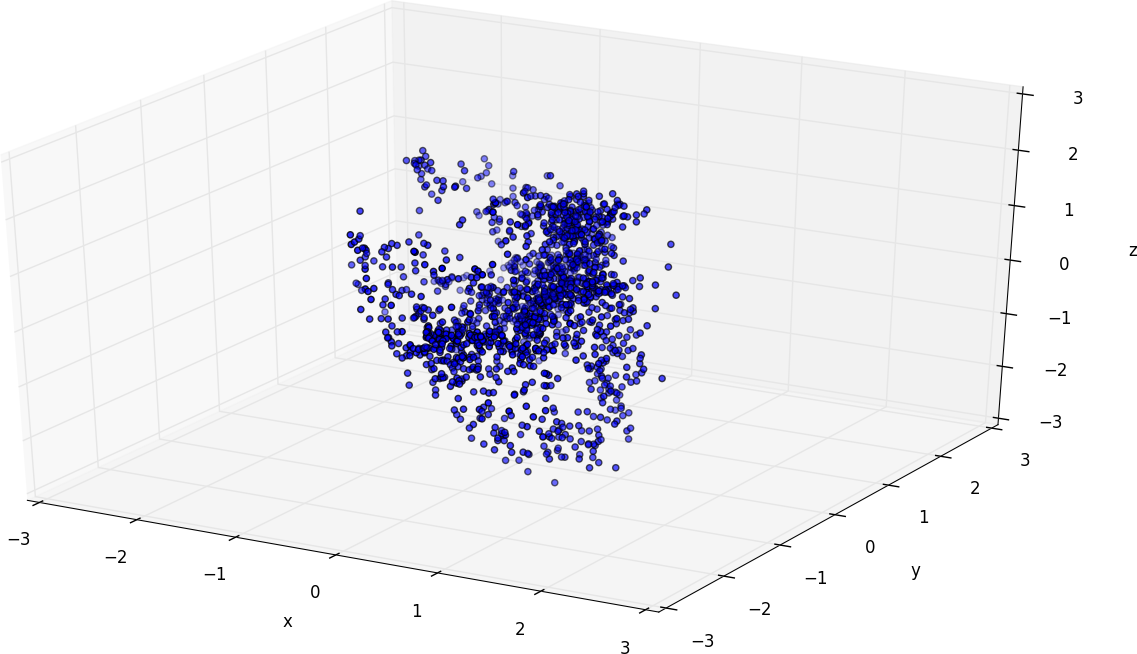
\includegraphics[width=\linewidth]{img/all.trimed.png}
%\caption{The first three dimension of a woman's MFCC feature}
%\end{minipage}
%\hfill
%\begin{minipage}{0.48\linewidth}
%\centering
%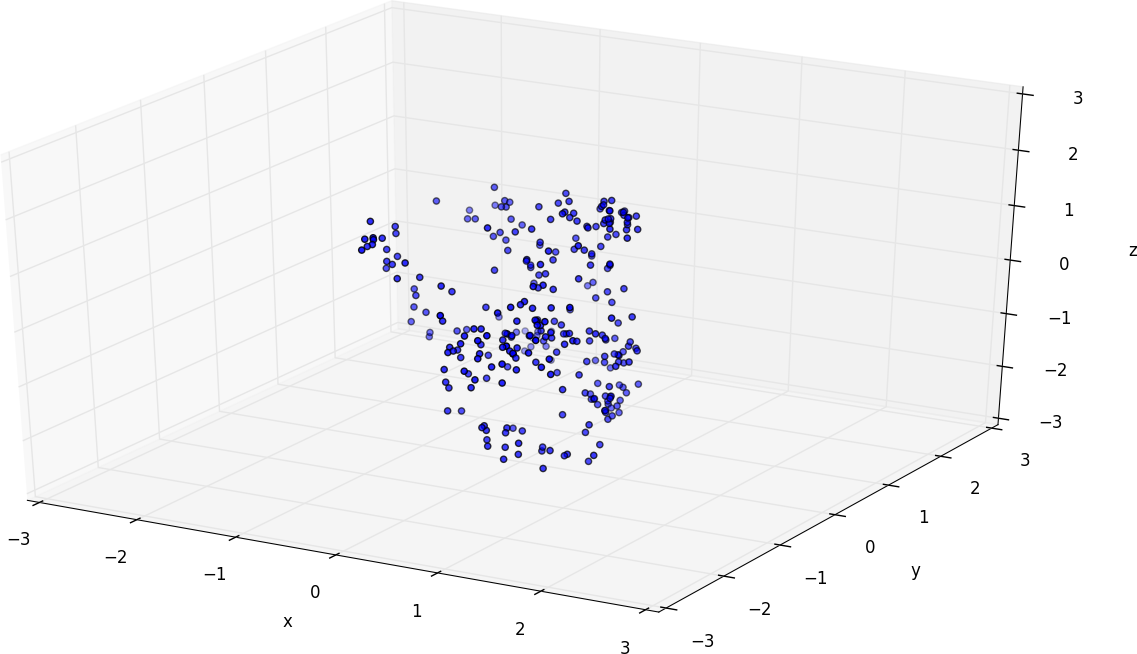
\includegraphics[width=\linewidth]{img/50.trimed.png}
%\caption{The first three dimension of the same woman's MFCC feature
%recontructed by a CRBM with 50-neuron hidden layer. We can
%see that, the density of these two distributions are alike}
%\end{minipage}
%\caption{\label{fig:crbm}}
%\end{figure}

%Here use CRBM as a substitution of GMM, rather than
%an feature extractor. We train a CRBM per speaker,
%and estimate reconstruction error without sampling (which is stable).
%The person corresponds to the lowest reconstruction error CRBM is adopted as
%recognition result.

%\item \textbf{JFA}:

%\textbf{Joint Factor Analysis} \cite{jfa2,jfa-se} was generally considered to perform better than other method
%in the task of Speaker Recognition, by modeling different types of variabilities in the training data, including session variability and
%speaker variability.

%Therefore, we use a simpler algorithm presented in \cite{jfa-study} to train the JFA model.
%However, the result shows that JFA does not seem to outperform GMM.
%We suspected that the training of a JFA model needs more data than
%we provided, since JFA needs data from various source to account for different types of variabilities.
%To get a higher accuracy in JFA, We might need to add extra data for training.
%\end{enumerate}

